\newpage\handout
{Part 1: electrostatics}
{\textsc{Electricity and Magnetism (E\&M)}}
{\href{https://creativecommons.org/licenses/by-nc-sa/4.0/}{CC BY-NC-SA 4.0 license}}
{Author: \BookAuthor}{Release: \generatedOn}
{E\&M: Part-1}
{\small\textbf{Purpose and Usage:}}\\[0.2cm]
{\footnotesize
These notes represent individual secondary work created by a TA at 
\WorksheetInstitution \space
based on experience with institutional course materials. While derived 
from \WorksheetInstitution \space
content, this compilation includes original explanations, 
examples, and pedagogical approaches developed independently. This work 
is shared as open source educational material and is not officially 
endorsed or authorized by \WorksheetInstitution.}\\[0.5cm]

{\small\textbf{For Educational Use:}}\\[0.2cm]
{\footnotesize
Students and educators are welcome to use and adapt these materials for 
non-commercial educational purposes. Please acknowledge both the original 
\WorksheetInstitution \space
source materials and the individual contributions of the 
author. This work is subject to removal or modification if \WorksheetInstitution 
determines it violates their Honor Code or intellectual property policies.}\\[0.5cm]

{\small\textbf{Content and Attribution:}}\\[0.2cm]
{\footnotesize
This work combines concepts and approaches learned through \WorksheetInstitution 
teaching experience with original pedagogical content. While inspired by 
institutional materials, all explanations, examples, and exercises are 
independently created. This compilation is shared under Creative Commons 
Attribution-NonCommercial-ShareAlike (CC BY-NC-SA) license, with proper 
attribution to both \WorksheetInstitution \space
and the individual author.}\\[0.5cm]

{\small\textbf{Quality Assurance:}}\\[0.2cm]
{\footnotesize
Efforts have been made to ensure clarity and correctness. Users are 
encouraged to verify concepts independently and report any errors or 
concerns. This work is provided as-is for educational benefit and 
may be subject to removal if institutional policies are violated.}

\begin{center}
  \includegraphics[width=0.30\textwidth]{\WorksheetEmblem}\\
  {\small © \the\year\ \BookAuthor. All rights reserved.}\\[0.5cm]
  {\small Prepared by \BookAuthor, TA@GT}\\[1cm]
\end{center}

\newpage
\newpage

\begin{enumerate}
  \item \textbf{Charge Distribution on Conducting Sphere} (10 points)\\
  A solid conducting sphere is given a positive charge $Q$. How is the charge $Q$ distributed in or on the sphere?
  \begin{enumerate}[label=(\Alph*)]
    \item It is concentrated at the center of the sphere.
    \item It is uniformly distributed throughout the sphere.
    \item Its density decreases radially outward from the center.
    \item It is uniformly distributed on the surface of the sphere only.
  \end{enumerate}
  \begin{subanswer}
    % your answer here
  \end{subanswer}

  \item \textbf{Parallel-Plate Capacitor Behavior} (10 points)\\
  A parallel-plate capacitor is charged by connection to a battery. If the battery is disconnected and the separation between the plates is increased, what will happen to the charge on the capacitor and the voltage across it?
  \begin{enumerate}[label=(\Alph*)]
    \item Both remain fixed.
    \item Both increase.
    \item The charge increases and the voltage decreases.
    \item The charge remains fixed and the voltage increases.
  \end{enumerate}
  \begin{subanswer}
    % your answer here
  \end{subanswer}

  \item \textbf{Work and Potential Difference} (10 points)\\
  One joule of work is needed to move one coulomb of charge from one point to another with no change in velocity. Which of the following is true between the two points?
  \begin{enumerate}[label=(\Alph*)]
    \item The current is one ampere.
    \item The potential difference is one volt.
    \item The electric field strength is one newton per coulomb.
    \item The electric field strength is one joule per electron.
  \end{enumerate}
  \begin{subanswer}
    % your answer here
  \end{subanswer}

  \item \textbf{Electric Field Magnitude} (10 points)\\
  \insertimage{0.40}{images/2025_07_25_f7c6487536cde8c1d115g-008}{Two positive charges of magnitude $q$ are each a distance $d$ from the origin $A$ of a coordinate system as shown above.}
  
  At which of the following points is the electric field least in magnitude?
  \begin{enumerate}[label=(\Alph*)]
    \item A
    \item B
    \item C
    \item D
  \end{enumerate}
  \begin{subanswer}
    % your answer here
  \end{subanswer}

  \item \textbf{Electric Potential Magnitude} (10 points)\\
  At which of the following points is the electric potential greatest in magnitude?
  \begin{enumerate}[label=(\Alph*)]
    \item A
    \item B
    \item C
    \item D
  \end{enumerate}
  \begin{subanswer}
    % your answer here
  \end{subanswer}

  \item \textbf{Capacitor Comparison} (10 points)\\
  A parallel-plate capacitor has a capacitance $C_0$. A second parallel-plate capacitor has plates with twice the area and twice the separation. The capacitance of the second capacitor is most nearly
  \begin{enumerate}[label=(\Alph*)]
    \item $\frac{1}{4}C_0$
    \item $C_0$
    \item $2C_0$
    \item $4C_0$
  \end{enumerate}
  \begin{subanswer}
    % your answer here
  \end{subanswer}

  \item \textbf{Charged Spheres Interaction} (10 points)\\
  \insertimage{0.40}{images/2025_07_25_f7c6487536cde8c1d115g-008(1)}{Two identical conducting spheres are charged to $+2Q$ and $-Q$, respectively, and are separated by a distance $d$ (much greater than the radii of the spheres) as shown above.}
  
  The magnitude of the force of attraction on the left sphere is $F_1$. After the two spheres are made to touch and then are re-separated by distance $d$, the magnitude of the force on the left sphere is $F_2$. Which of the following relationships is correct?
  \begin{enumerate}[label=(\Alph*)]
    \item $2F_1 = F_2$
    \item $F_1 = F_2$
    \item $F_1 = 2F_2$
    \item $F_1 = 8F_2$
  \end{enumerate}
  \begin{subanswer}
    % your answer here
  \end{subanswer}

  \item \textbf{Capacitance Factors} (10 points)\\
  The capacitance of a parallel-plate capacitor can be increased by increasing which of the following?
  \begin{enumerate}[label=(\Alph*)]
    \item The distance between the plates
    \item The charge on each plate
    \item The area of the plates
    \item The potential difference across the plates
  \end{enumerate}
  \begin{subanswer}
    % your answer here
  \end{subanswer}

  \item \textbf{Hollow Metal Sphere Electric Field} (10 points)\\
  A hollow metal sphere of radius $R$ is positively charged. Of the following distances from the center of the sphere, which location will have the greatest electric field strength?
  \begin{enumerate}[label=(\Alph*)]
    \item 0 (center of the sphere)
    \item $\frac{3R}{2}$
    \item $2R$
    \item None of the above because the field is of constant strength
  \end{enumerate}
  \begin{subanswer}
    % your answer here
  \end{subanswer}

  \item \textbf{Force Between Charges} (10 points)\\
  Two isolated charges, $+q$ and $-2q$, are 2 centimeters apart. If $F$ is the magnitude of the force acting on charge $-2q$, what are the magnitude and direction of the force acting on charge $+q$?
  
  \begin{center}
  \begin{tabular}{|l|l|}
  \hline
  \textbf{Magnitude} & \textbf{Direction} \\
  \hline
  (A) $\frac{1}{2}F$ & Toward charge $-2q$ \\
  (B) $2F$ & Away from charge $-2q$ \\
  (C) $F$ & Toward charge $-2q$ \\
  (D) $F$ & Away from charge $-2q$ \\
  \hline
  \end{tabular}
  \end{center}
  \begin{subanswer}
    % your answer here
  \end{subanswer}

  \item \textbf{Net Electric Field Zero} (10 points)\\
  \insertimage{0.40}{images/2025_07_25_f7c6487536cde8c1d115g-009}{Charges $+Q$ and $-4Q$ are situated as shown above.}
  
  The net electric field is zero nearest which point?
  \begin{enumerate}[label=(\Alph*)]
    \item A
    \item C
    \item D
    \item E
  \end{enumerate}
  \begin{subanswer}
    % your answer here
  \end{subanswer}

  \item \textbf{Charged Conducting Sphere Properties} (10 points)\\
  A positive charge of $10^{-6}$ coulomb is placed on an insulated solid conducting sphere. Which of the following is true?
  \begin{enumerate}[label=(\Alph*)]
    \item The charge resides uniformly throughout the sphere.
    \item The electric field in the region surrounding the sphere increases with increasing distance from the sphere.
    \item An insulated metal object acquires a net positive charge when brought near to, but not in contact with, the sphere.
    \item When a second conducting sphere is connected by a conducting wire to the first sphere, charge is transferred until the electric potentials of the two spheres are equal.
  \end{enumerate}
  \begin{subanswer}
    % your answer here
  \end{subanswer}

  \item \textbf{Parallel Plates Force Comparison} (10 points)\\
  \insertimage{0.40}{images/2025_07_25_f7c6487536cde8c1d115g-009(1)}{Two large parallel conducting plates P and Q are connected to a battery of emf $\mathcal{E}$, as shown above.}
  
  A test charge is placed successively at points I, II, and III. If edge effects are negligible, the force on the charge when it is at point III is
  \begin{enumerate}[label=(\Alph*)]
    \item of equal magnitude and in the same direction as the force on the charge when it is at point I
    \item of equal magnitude and in the same direction as the force on the charge when it is at point II
    \item much greater in magnitude than the force on the charge when it is at point II, but in the same direction
    \item much less in magnitude than the force on the charge when it is at point II, but in the same direction
  \end{enumerate}
  \begin{subanswer}
    % your answer here
  \end{subanswer}

  \item \textbf{Electric Field Ratio} (10 points)\\
  \insertimage{0.40}{images/2025_07_25_f7c6487536cde8c1d115g-010(2)}{The diagram above shows an isolated, positive charge $Q$. Point $B$ is twice as far away from $Q$ as point $A$.}
  
  The ratio of the electric field strength at point $A$ to the electric field strength at point $B$ is
  \begin{enumerate}[label=(\Alph*)]
    \item 8 to 1
    \item 4 to 1
    \item 2 to 1
    \item 1 to 2
  \end{enumerate}
  \begin{subanswer}
    % your answer here
  \end{subanswer}

  \item \textbf{Uncharged Sphere in Electric Field} (10 points)\\
  Which of the following is true about the net force on an uncharged conducting sphere in a uniform electric field?
  \begin{enumerate}[label=(\Alph*)]
    \item It is zero.
    \item It is in the direction of the field.
    \item It is in the direction opposite to the field.
    \item It causes the sphere to oscillate about an equilibrium position.
  \end{enumerate}
  \begin{subanswer}
    % your answer here
  \end{subanswer}

  \item \textbf{Conducting Spheres Charge Flow} (10 points)\\
  \insertimage{0.40}{images/2025_07_25_f7c6487536cde8c1d115g-010(5)}{Two conducting spheres of different radii, as shown above, each have charge $-Q$.}
  
  Which of the following occurs when the two spheres are connected with a conducting wire?
  \begin{enumerate}[label=(\Alph*)]
    \item No charge flows.
    \item Negative charge flows from the larger sphere to the smaller sphere until the electric potential of each sphere is the same.
    \item Negative charge flows from the smaller sphere to the larger sphere until the electric field at the surface of each sphere is the same.
    \item Negative charge flows from the smaller sphere to the larger sphere until the electric potential of each sphere is the same.
  \end{enumerate}
  \begin{subanswer}
    % your answer here
  \end{subanswer}

  \item \textbf{Electric Field Calculation} (10 points)\\
  Two parallel conducting plates are connected to a constant voltage source. The magnitude of the electric field between the plates is $2,000$ N/C. If the voltage is doubled and the distance between the plates is reduced to $\frac{1}{5}$ the original distance, the magnitude of the new electric field is
  \begin{enumerate}[label=(\Alph*)]
    \item $800$ N/C
    \item $1,600$ N/C
    \item $2,400$ N/C
    \item $20,000$ N/C
  \end{enumerate}
  \begin{subanswer}
    % your answer here
  \end{subanswer}

  \item \textbf{Square Configuration Electric Field} (10 points)\\
  \insertimage{0.40}{images/2025_07_25_f7c6487536cde8c1d115g-010(1)}{The figure above shows two particles, each with a charge of $+Q$, that are located at the opposite corners of a square of side $d$.}
  
  What is the direction of the net electric field at point P?
  \begin{center}
  \begin{tabular}{cccc}
  A. & B. & C. & D. \\
  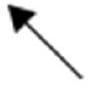
\includegraphics[width=0.15\textwidth]{images/2025_07_25_f7c6487536cde8c1d115g-010(3)} &
  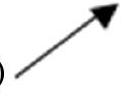
\includegraphics[width=0.15\textwidth]{images/2025_07_25_f7c6487536cde8c1d115g-010(4)} &
  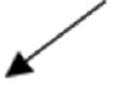
\includegraphics[width=0.15\textwidth]{images/2025_07_25_f7c6487536cde8c1d115g-010} &
  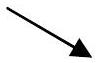
\includegraphics[width=0.15\textwidth]{images/2025_07_25_f7c6487536cde8c1d115g-011} \\
  \end{tabular}
  \end{center}
  \begin{subanswer}
    % your answer here
  \end{subanswer}

  \item \textbf{Potential Energy Calculation} (10 points)\\
  What is the potential energy of a particle of charge $+q$ that is held at point P?
  \begin{enumerate}[label=(\Alph*)]
    \item Zero
    \item $\frac{\sqrt{2}}{4\pi\varepsilon_0}\frac{qQ}{d}$
    \item $\frac{2}{4\pi\varepsilon_0}\frac{qQ}{d}$
    \item $\frac{2\sqrt{2}}{4\pi\varepsilon_0}\frac{qQ}{d}$
  \end{enumerate}
  \begin{subanswer}
    % your answer here
  \end{subanswer}

  \item \textbf{Plate Separation Effect} (10 points)\\
  Two parallel conducting plates, separated by a distance $d$, are connected to a battery of emf $\varepsilon$. Which of the following is correct if the plate separation is doubled while the battery remains connected?
  \begin{enumerate}[label=(\Alph*)]
    \item The electric charge on the plates is doubled.
    \item The electric charge on the plates is halved.
    \item The potential difference between the plates is doubled.
    \item The capacitance is unchanged.
  \end{enumerate}
  \begin{subanswer}
    % your answer here
  \end{subanswer}

  \item \textbf{Hollow Metal Sphere Electric Field} (10 points)\\
  \insertimage{0.40}{images/2025_07_25_f7c6487536cde8c1d115g-011(3)}{The hollow metal sphere shown above is positively charged. Point C is the center of the sphere and point P is any other point within the sphere.}
  
  Which of the following is true of the electric field at these points?
  \begin{enumerate}[label=(\Alph*)]
    \item It is zero at both points.
    \item It is zero at C, but at P it is not zero and is directed inward.
    \item It is zero at C, but at P it is not zero and is directed outward.
    \item It is not zero at either point.
  \end{enumerate}
  \begin{subanswer}
    % your answer here
  \end{subanswer}

  \item \textbf{Coordinate System Electric Field} (10 points)\\
  \insertimage{0.40}{images/2025_07_25_f7c6487536cde8c1d115g-011(4)}{Charges $-Q$ and $+Q$ are located on the $x$- and $y$-axes, respectively, each at a distance $d$ from the origin $O$, as shown above.}
  
  What is the direction of the electric field at the origin $O$?
  \begin{center}
  \begin{tabular}{cccc}
  A. & B. & C. & D. \\
  $\longrightarrow$ &
  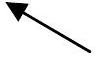
\includegraphics[width=0.15\textwidth]{images/2025_07_25_f7c6487536cde8c1d115g-011(2)} &
  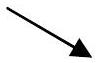
\includegraphics[width=0.15\textwidth]{images/2025_07_25_f7c6487536cde8c1d115g-011} &
  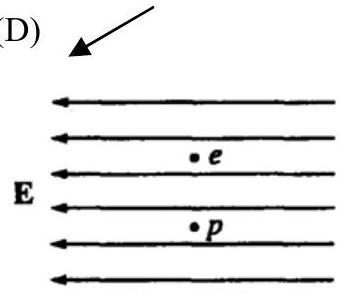
\includegraphics[width=0.15\textwidth]{images/2025_07_25_f7c6487536cde8c1d115g-011(1)} \\
  \end{tabular}
  \end{center}
  \begin{subanswer}
    % your answer here
  \end{subanswer}

  \item \textbf{Electron and Proton in Electric Field} (10 points)\\
  An electron $e$ and a proton $p$ are simultaneously released from rest in a uniform electric field $E$, as shown above. Assume that the particles are sufficiently far apart so that the only force acting on each particle after it is released is that due to the electric field. At a later time when the particles are still in the field, the electron and the proton will have the same
  \begin{enumerate}[label=(\Alph*)]
    \item direction of motion
    \item speed
    \item magnitude of acceleration
    \item magnitude of force acting on them
  \end{enumerate}
  \begin{subanswer}
    % your answer here
  \end{subanswer}

  \item \textbf{Electric Potential at Point} (10 points)\\
  \insertimage{0.40}{images/2025_07_25_f7c6487536cde8c1d115g-011(5)}{Two large, flat, parallel, conducting plates are 0.04 m apart, as shown above. The lower plate is at a potential of 2 V with respect to ground. The upper plate is at a potential of 10 V with respect to ground. Point $P$ is located 0.01 m above the lower plate.}
  
  The electric potential at point $P$ is
  \begin{enumerate}[label=(\Alph*)]
    \item 10 V
    \item 8 V
    \item 6 V
    \item 4 V
  \end{enumerate}
  \begin{subanswer}
    % your answer here
  \end{subanswer}

  \item \textbf{Kinetic Energy Comparison} (10 points)\\
  A particle of charge $Q$ and mass $m$ is accelerated from rest through a potential difference $V$, attaining a kinetic energy $K$. What is the kinetic energy of a particle of charge $2Q$ and mass $\frac{m}{2}$ that is accelerated from rest through the same potential difference?
  \begin{enumerate}[label=(\Alph*)]
    \item $\frac{1}{2}K$
    \item $K$
    \item $2K$
    \item $4K$
  \end{enumerate}
  \begin{subanswer}
    % your answer here
  \end{subanswer}

  \item \textbf{Electric Field Lines Analysis} (10 points)\\
  \insertimage{0.40}{images/2025_07_25_f7c6487536cde8c1d115g-012(1)}{The diagram above shows electric field lines in an isolated region of space containing two small charged spheres, $Y$ and $Z$.}
  
  Which of the following statements is true?
  \begin{enumerate}[label=(\Alph*)]
    \item The charge on $Y$ is negative and the charge on $Z$ is positive.
    \item The strength of the electric field is the same everywhere.
    \item The electric field is strongest midway between $Y$ and $Z$.
    \item A small negatively charged object placed at point $X$ would tend to move toward the right.
  \end{enumerate}
  \begin{subanswer}
    % your answer here
  \end{subanswer}

  \item \textbf{Capacitor Comparison} (10 points)\\
  A parallel-plate capacitor has a capacitance $C_0$. A second parallel-plate capacitor has plates with twice the area and twice the separation. The capacitance of the second capacitor is most nearly
  \begin{enumerate}[label=(\Alph*)]
    \item $\frac{1}{4}C_0$
    \item $\frac{1}{2}C_0$
    \item $C_0$
    \item $2C_0$
  \end{enumerate}
  \begin{subanswer}
    % your answer here
  \end{subanswer}

  \item \textbf{Electric Field Near Conductor} (10 points)\\
  The electric field $E$ just outside the surface of a charged conductor is
  \begin{enumerate}[label=(\Alph*)]
    \item directed perpendicular to the surface
    \item directed parallel to the surface
    \item zero
    \item infinite
  \end{enumerate}
  \begin{subanswer}
    % your answer here
  \end{subanswer}

  \item \textbf{Work Required for Charge Movement} (10 points)\\
  \insertimage{0.40}{images/2025_07_25_f7c6487536cde8c1d115g-012}{Points R and S are each the same distance $d$ from two unequal charges, $+Q$ and $+2Q$, as shown above.}
  
  The work required to move a charge $-Q$ from point R to point S is
  \begin{enumerate}[label=(\Alph*)]
    \item dependent on the path taken from R to S
    \item positive
    \item zero
    \item negative
  \end{enumerate}
  \begin{subanswer}
    % your answer here
  \end{subanswer}

  \item \textbf{Rigid Rod in Electric Field} (10 points)\\
  \insertimage{0.40}{images/2025_07_25_f7c6487536cde8c1d115g-012(2)}{A rigid insulated rod, with two unequal charges attached to its ends, is placed in a uniform electric field $E$ as shown above.}
  
  The rod experiences a
  \begin{enumerate}[label=(\Alph*)]
    \item net force to the left and a clockwise rotation
    \item net force to the left and a counterclockwise rotation
    \item net force to the right and a clockwise rotation
    \item net force to the right and a counterclockwise rotation
  \end{enumerate}
  \begin{subanswer}
    % your answer here
  \end{subanswer}

  \item \textbf{Coaxial Cylinders Charge} (10 points)\\
  \insertimage{0.40}{images/2025_07_25_f7c6487536cde8c1d115g-013(4)}{The electric field of two long coaxial cylinders is represented by lines of force as shown above. The charge on the inner cylinder is $+Q$.}
  
  The charge on the outer cylinder is
  \begin{enumerate}[label=(\Alph*)]
    \item $+3Q$
    \item $+Q$
    \item $-Q$
    \item $-3Q$
  \end{enumerate}
  \begin{subanswer}
    % your answer here
  \end{subanswer}

  \item \textbf{Capacitor with Dielectric} (10 points)\\
  An isolated capacitor with air between its plates has a potential difference $V_0$ and a charge $Q_0$. After the space between the plates is filled with oil, the difference in potential is $V$ and the charge is $Q$. Which of the following pairs of relationships is correct?
  \begin{enumerate}[label=(\Alph*)]
    \item $Q = Q_0$ and $V > V_0$
    \item $Q = Q_0$ and $V < V_0$
    \item $Q > Q_0$ and $V = V_0$
    \item $Q < Q_0$ and $V < V_0$
  \end{enumerate}
  \begin{subanswer}
    % your answer here
  \end{subanswer}

  \item \textbf{Coulomb's Law Application} (10 points)\\
  Two small spheres have equal charges $q$ and are separated by a distance $d$. The force exerted on each sphere by the other has magnitude $F$. If the charge on each sphere is doubled and $d$ is halved, the force on each sphere has magnitude
  \begin{enumerate}[label=(\Alph*)]
    \item $F$
    \item $4F$
    \item $8F$
    \item $16F$
  \end{enumerate}
  \begin{subanswer}
    % your answer here
  \end{subanswer}

  \item \textbf{Conductors Under Electrostatic Conditions} (10 points)\\
  Which of the following statements about conductors under electrostatic conditions is true?
  \begin{enumerate}[label=(\Alph*)]
    \item Positive work is required to move a positive charge over the surface of a conductor.
    \item Charge that is placed on the surface of a conductor always spreads evenly over the surface.
    \item The electric potential inside a conductor is always zero.
    \item The surface of a conductor is always an equipotential surface.
  \end{enumerate}
  \begin{subanswer}
    % your answer here
  \end{subanswer}

  \item \textbf{Charged Particle Force Direction} (10 points)\\
  A charged particle traveling with a velocity $v$ in an electric field $E$ experiences a force $F$ that must be
  \begin{enumerate}[label=(\Alph*)]
    \item parallel to $v$
    \item perpendicular to $v$
    \item parallel to $E$
    \item perpendicular to $E$
  \end{enumerate}
  \begin{subanswer}
    % your answer here
  \end{subanswer}

  \item \textbf{Work Done by Electric Force} (10 points)\\
  A positive charge of $3.0 \times 10^{-8}$ coulomb is placed in an upward directed uniform electric field of $4.0 \times 10^4$ N/C. When the charge is moved 0.5 meter upward, the work done by the electric force on the charge is
  \begin{enumerate}[label=(\Alph*)]
    \item $6 \times 10^{-4}$ J
    \item $12 \times 10^{-4}$ J
    \item $2 \times 10^4$ J
    \item $8 \times 10^4$ J
  \end{enumerate}
  \begin{subanswer}
    % your answer here
  \end{subanswer}

  \item \textbf{Equilateral Triangle Configurations} (10 points)\\
  The following configurations of electric charges are located at the vertices of an equilateral triangle. Point $P$ is equidistant from the charges.
  \begin{center}
  \begin{tabular}{cccc}
  A. & B. & C. & D. \\
  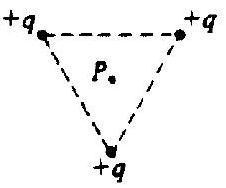
\includegraphics[width=0.15\textwidth]{images/2025_07_25_f7c6487536cde8c1d115g-013(1)} &
  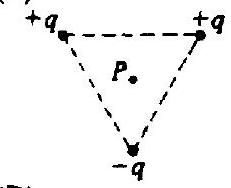
\includegraphics[width=0.15\textwidth]{images/2025_07_25_f7c6487536cde8c1d115g-013} &
  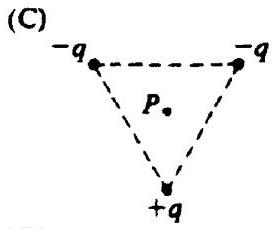
\includegraphics[width=0.15\textwidth]{images/2025_07_25_f7c6487536cde8c1d115g-013(2)} &
  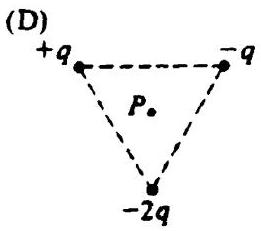
\includegraphics[width=0.15\textwidth]{images/2025_07_25_f7c6487536cde8c1d115g-013(3)} \\
  \end{tabular}
  \end{center}
  
  In which configuration is the electric field at P equal to zero?
  \begin{enumerate}[label=(\Alph*)]
    \item A
    \item B
    \item C
    \item D
  \end{enumerate}
  \begin{subanswer}
    % your answer here
  \end{subanswer}

  \item \textbf{Electric Field Direction in Triangle} (10 points)\\
  In which configuration is the electric field at P pointed at the midpoint between two of the charges?
  \begin{enumerate}[label=(\Alph*)]
    \item A
    \item B
    \item C
    \item D
  \end{enumerate}
  \begin{subanswer}
    % your answer here
  \end{subanswer}

  \item \textbf{Mica Sheet in Capacitor} (10 points)\\
  A sheet of mica is inserted between the plates of an isolated charged parallel-plate capacitor. Which of the following statements is true?
  \begin{enumerate}[label=(\Alph*)]
    \item The capacitance decreases.
    \item The potential difference across the capacitor decreases.
    \item The charge on the capacitor plates decreases.
    \item The electric field between the capacitor plates increases.
  \end{enumerate}
  \begin{subanswer}
    % your answer here
  \end{subanswer}

  \item \textbf{Conducting Spheres Electron Flow} (10 points)\\
  \insertimage{0.40}{images/2025_07_25_f7c6487536cde8c1d115g-014}{Two conducting spheres, $X$ and $Y$ have the same positive charge $+Q$, but different radii $(r_x > r_y)$ as shown above. The spheres are separated so that the distance between them is large compared with either radius.}
  
  If a wire is connected between them, in which direction will electrons be directed in the wire?
  \begin{enumerate}[label=(\Alph*)]
    \item From X to Y
    \item From Y to X
    \item There will be no flow of charge in the wire.
    \item It cannot be determined without knowing the magnitude of Q.
  \end{enumerate}
  \begin{subanswer}
    % your answer here
  \end{subanswer}

  \item \textbf{Charged Sphere Inside Field} (10 points)\\
  A sphere of radius $R$ has positive charge $Q$ uniformly distributed on its surface.
  
  Which of the following represents the magnitude of the electric field $E$ and the potential $V$ as functions of $r$, the distance from the center of the sphere, when $r < R$?
  
  \begin{center}
  \begin{tabular}{|l|l|l|}
  \hline
  & $\underline{E}$ & $\underline{V}$ \\
  \hline
  (A) & 0 & 0 \\
  (B) & 0 & $kQ/R$ \\
  (C) & $kQ/r^2$ & 0 \\
  (D) & $kQ/R^2$ & 0 \\
  \hline
  \end{tabular}
  \end{center}
  \begin{subanswer}
    % your answer here
  \end{subanswer}

  \item \textbf{Charged Sphere Outside Field} (10 points)\\
  Which of the following represents the magnitude of the electric field $E$ and the potential $V$ as functions of $r$, the distance from the center of sphere, when $r > R$?
  
  \begin{center}
  \begin{tabular}{|l|l|l|}
  \hline
  & $\underline{E}$ & $\underline{V}$ \\
  \hline
  (A) & $kQ/R^2$ & $kQ/R$ \\
  (B) & $kQ/R$ & $kQ/r$ \\
  (C) & $kQ/r^2$ & $kQ/r$ \\
  (D) & $kQ/r^2$ & $kQ/r^2$ \\
  \hline
  \end{tabular}
  \end{center}
  \begin{subanswer}
    % your answer here
  \end{subanswer}

  \item \textbf{Electric Field Vector Properties} (10 points)\\
  From the electric field vector at a point, one can determine which of the following?
  \begin{enumerate}[label=(\Roman*)]
    \item The direction of the electrostatic force on a test charge of known sign at that point
    \item The magnitude of the electrostatic force exerted per unit charge on a test charge at that point
    \item The electrostatic charge at that point
  \end{enumerate}
  \begin{enumerate}[label=(\Alph*)]
    \item I only
    \item III only
    \item I and II only
    \item II and III only
  \end{enumerate}
  \begin{subanswer}
    % your answer here
  \end{subanswer}

  \item \textbf{Conducting Spheres Field Ratio} (10 points)\\
  A conducting sphere of radius $R$ carries a charge $Q$. Another conducting sphere has a radius $R/2$, but carries the same charge. The spheres are far apart. The ratio of the electric field near the surface of the smaller sphere to the field near the surface of the larger sphere is most nearly
  \begin{enumerate}[label=(\Alph*)]
    \item $\frac{1}{4}$
    \item $\frac{1}{2}$
    \item 2
    \item 4
  \end{enumerate}
  \begin{subanswer}
    % your answer here
  \end{subanswer}

  \item \textbf{Circular Ring Charge Distribution} (10 points)\\
  \insertimage{0.40}{images/2025_07_25_f7c6487536cde8c1d115g-015(3)}{A circular ring made of an insulating material is cut in half. One half is given a charge $-q$ uniformly distributed along its arc. The other half is given a charge $+q$ also uniformly distributed along its arc. The two halves are then rejoined with insulation at the junctions J, as shown above.}
  
  If there is no change in the charge distributions, what is the direction of the net electrostatic force on an electron located at the center of the circle?
  \begin{enumerate}[label=(\Alph*)]
    \item Toward the top of the page
    \item Toward the bottom of the page
    \item To the right
    \item To the left
  \end{enumerate}
  \begin{subanswer}
    % your answer here
  \end{subanswer}

  \item \textbf{Square Charge Configuration} (10 points)\\
  \insertimage{0.40}{images/2025_07_25_f7c6487536cde8c1d115g-015}{Four positive charges of magnitude $q$ are arranged at the corners of a square, as shown above. At the center C of the square, the potential due to one charge alone is $V_0$ and the electric field due to one charge alone has magnitude $E_0$.}
  
  Which of the following correctly gives the electric potential and the magnitude of the electric field at the center of the square due to all four charges?
  
  \begin{center}
  \begin{tabular}{|l|l|l|}
  \hline
  & \textbf{Electric Potential} & \textbf{Electric Field} \\
  \hline
  (A) & Zero & Zero \\
  (B) & Zero & $2E_0$ \\
  (C) & $4V_0$ & Zero \\
  (D) & $4V_0$ & $2E_0$ \\
  \hline
  \end{tabular}
  \end{center}
  \begin{subanswer}
    % your answer here
  \end{subanswer}

  \item \textbf{Electric Potential Zero Points} (10 points)\\
  \insertimage{0.40}{images/2025_07_25_f7c6487536cde8c1d115g-015(2)}{Two charges, $-2Q$ and $+Q$, are located on the $x$-axis, as shown above. Point P, at a distance of $3D$ from the origin O, is one of two points on the positive $x$-axis at which the electric potential is zero.}
  
  How far from the origin O is the other point?
  \begin{enumerate}[label=(\Alph*)]
    \item $\frac{2}{3}D$
    \item $\frac{3}{2}D$
    \item $\frac{5}{3}D$
    \item $2D$
  \end{enumerate}
  \begin{subanswer}
    % your answer here
  \end{subanswer}

  \item \textbf{Concentric Spherical Shells} (10 points)\\
  \insertimage{0.40}{images/2025_07_25_f7c6487536cde8c1d115g-015(1)}{Two concentric, spherical conducting shells have radii $r_1$ and $r_2$ and charges $Q_1$ and $Q_2$, as shown above. Let $r$ be the distance from the center of the spheres and consider the region $r_1 < r < r_2$.}
  
  In this region the electric field is proportional to
  \begin{enumerate}[label=(\Alph*)]
    \item $Q_1/r^2$
    \item $(Q_1 + Q_2)/r^2$
    \item $(Q_1 + Q_2)/r$
    \item $Q_1/r + Q_2/r_2$
  \end{enumerate}
  \begin{subanswer}
    % your answer here
  \end{subanswer}

  \item \textbf{Equipotential Lines Configuration} (10 points)\\
  \insertimage{0.40}{images/2025_07_25_f7c6487536cde8c1d115g-016(3)}{A battery or batteries connected to two parallel plates produce the equipotential lines between the plates shown above.}
  
  Which of the following configurations is most likely to produce these equipotential lines?
  \begin{center}
  \begin{tabular}{cccc}
  A. & B. & C. & D. \\
  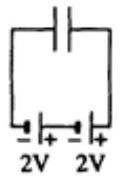
\includegraphics[width=0.15\textwidth]{images/2025_07_25_f7c6487536cde8c1d115g-016(5)} &
  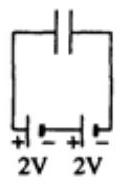
\includegraphics[width=0.15\textwidth]{images/2025_07_25_f7c6487536cde8c1d115g-016(4)} &
  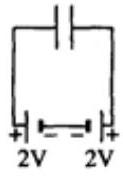
\includegraphics[width=0.15\textwidth]{images/2025_07_25_f7c6487536cde8c1d115g-016} &
  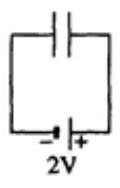
\includegraphics[width=0.15\textwidth]{images/2025_07_25_f7c6487536cde8c1d115g-016(1)} \\
  \end{tabular}
  \end{center}
  \begin{subanswer}
    % your answer here
  \end{subanswer}

  \item \textbf{Force on Electron at Zero Potential} (10 points)\\
  \insertimage{0.40}{images/2025_07_25_f7c6487536cde8c1d115g-016(2)}{The force on an electron located on the 0 volt potential line is}
  
  \begin{enumerate}[label=(\Alph*)]
    \item 0 N
    \item 1 N, directed to the right
    \item 1 N, directed to the left
    \item to the right, but its magnitude cannot be determined without knowing the distance between the lines
  \end{enumerate}
  \begin{subanswer}
    % your answer here
  \end{subanswer}

  \item \textbf{Charging by Induction} (10 points)\\
  \insertimage{0.40}{images/2025_07_25_f7c6487536cde8c1d115g-016(2)}{Two metal spheres that are initially uncharged are mounted on insulating stands, as shown above. A negatively charged rubber rod is brought close to, but does not make contact with, sphere X. Sphere Y is then brought close to X on the side opposite to the rubber rod. Y is allowed to touch X and then is removed some distance away. The rubber rod is then moved far away from $X$ and $Y$.}
  
  What are the final charges on the spheres?
  
  \begin{center}
  \begin{tabular}{|l|l|l|}
  \hline
  & \textbf{Sphere X} & \textbf{Sphere Y} \\
  \hline
  (A) & Zero & Zero \\
  (B) & Negative & Positive \\
  (C) & Positive & Negative \\
  (D) & Positive & Positive \\
  \hline
  \end{tabular}
  \end{center}
  \begin{subanswer}
    % your answer here
  \end{subanswer}
\end{enumerate}

